% !TEX TS-program = pdflatex
% !TEX encoding = UTF-8 Unicode

% This file is a template using the "beamer" package to create slides for a talk or presentation
% - Giving a talk on some subject.
% - The talk is between 15min and 45min long.
% - Style is ornate.

% MODIFIED by Jonathan Kew, 2008-07-06
% The header comments and encoding in this file were modified for inclusion with TeXworks.
% The content is otherwise unchanged from the original distributed with the beamer package.

\documentclass{beamer}


% Copyright 2004 by Till Tantau <tantau@users.sourceforge.net>.
%
% In principle, this file can be redistributed and/or modified under
% the terms of the GNU Public License, version 2.
%
% However, this file is supposed to be a template to be modified
% for your own needs. For this reason, if you use this file as a
% template and not specifically distribute it as part of a another
% package/program, I grant the extra permission to freely copy and
% modify this file as you see fit and even to delete this copyright
% notice. 


\mode<presentation>
{
  \usetheme{Berkeley}
  % or ...

  \setbeamercovered{transparent}
  % or whatever (possibly just delete it)
}

\usepackage{tikz}
\usepackage{graphicx}
\graphicspath{{C:/Users/garret/GoogleDrive/CEGA/CEGA-Programs/BITSS/Supporting-Material-Slides/APHRC/Images/}}
\usepackage[english]{babel}
% or whatever

\usepackage[utf8]{inputenc}
% or whatever

\usepackage{times}
\usepackage[T1]{fontenc}
% Or whatever. Note that the encoding and the font should match. If T1
% does not look nice, try deleting the line with the fontenc.


\title[Short Paper Title] % (optional, use only with long paper titles)
{Software and Workflow for Reproducible Research}

\subtitle
{Discussion} % (optional)

\author[Christensen] % (optional, use only with lots of authors)
{Garret Christensen\inst{1}}
% - Use the \inst{?} command only if the authors have different
%   affiliation.

\institute[UC Berkeley, Berkely Initiatiative for Transparency in the Social Sciences] % (optional, but mostly needed)
{
  \inst{1}%
  UC Berkeley: Berkely Initiatiative for Transparency in the Social Sciences\\
  Berkeley Institute for Data Science
}
% - Use the \inst command only if there are several affiliations.
% - Keep it simple, no one is interested in your street address.

\date[Short Occasion] % (optional)
{APHRC, Summer 2015}

\subject{Talks}
% This is only inserted into the PDF information catalog. Can be left
% out. 

\pgfdeclareimage[height=2cm]{university-logo}{C:/Users/garret/GoogleDrive/CEGA/CEGA-Programs/BITSS/Supporting-Material-Slides/APHRC/Images/BITSSlogo.png}
 \logo{\pgfuseimage{university-logo}}

% Delete this, if you do not want the table of contents to pop up at
% the beginning of each subsection:
%\AtBeginSubsection[]
%{
%  \begin{frame}<beamer>{Outline}
%   \tableofcontents[currentsection,currentsubsection]
%  \end{frame}
%}


% If you wish to uncover everything in a step-wise fashion, uncomment
% the following command: 

%\beamerdefaultoverlayspecification{<+->}

\begin{document}

% Since this a solution template for a generic talk, very little can
% be said about how it should be structured. However, the talk length
% of between 15min and 45min and the theme suggest that you stick to
% the following rules:  

% - Exactly two or three sections (other than the summary).
% - At *most* three subsections per section.
% - Talk about 30s to 2min per frame. So there should be between about
%   15 and 30 frames, all told.

\begin{frame}
  \titlepage
\end{frame}

\begin{frame}

\includegraphics[height=0.75in]{BITSSlogo.PNG}

 \url{bitss.org}
 
\end{frame}

\begin{frame}{Outline}
  \tableofcontents
  % You might wish to add the option [pausesections]
\end{frame}


\section{Introduction}
\begin{frame}{Reproducibility \& Transparency}
\begin{itemize}
\item What are problems associated with reproducibility?
\item What are solutions to these problems?
\item What are practical tools to implement these solutions?
\end{itemize}
\end{frame}
%%%%%%%%%%%%%%%%%%%%%%%%%%%%%%%%%%%%%%%%%%%%%%%%%%%%%%%%%%%%%%%%%%
\section{Problems}
\begin{frame}{Problems}
 \begin{itemize}
 \item Publication bias (see previous talk)
 \item Specification Searching (see previous talk)
 \item Data not available
 \item Code not available/unintelligible
 \end{itemize}
\end{frame}

 
\subsection{Irreproducible Workflow}
 \begin{frame}{Irreproducible Workflow}
 \begin{itemize}
 \item
  Even with the original authors' help, you can't get the data to reproduce the published results. Or you just can't find the data to begin with. 
  \item \textit{Journal of Money, Credit, and Banking} Project. \href{http://www.jstor.org/stable/1806061}{(Dewald et al., AER 1986)}
   \item Martin Feldstein on Social Security and private savings, Reinhart and Rogoff on debt and GDP growth.
 \end{itemize} 
 \end{frame}
%%%%%%%%%%%%%%%%%%%%%%%%%%%%%%%%%%%%%%%%%%%%%%%%%%%%%%%%%%%%%%%%%%%%

\section{Solutions}
\begin{frame}{Solutions}
\begin{itemize}[<+->]
\item Study Registry (see previous talk)
\item Pre-Analysis Plan (see previous talk)
\item Reproducible Workflow
 \begin{itemize}
 \item Literate Programing 
 \item Data Sharing
 \end{itemize}
\end{itemize}
\end{frame}

%%%%%%%%%%%%%%%%%%%%%%%%%%%%%%%%%%%%%%%%%%%%%%%%%%%%%%%%%%%%%%%%%%%%%

\subsection{Workflow}
\begin{frame}{Reproducible Workflow}
 \begin{itemize}
 \item R Markdown and \href{http://rstudio.com}{R Studio} to write dynamic documents.
 \item Version control with \href{http://www.github.com}{Github} or \href{http://osf.io}{OSF}. 
 \item Literate Programing
  \begin{itemize}
   \item Writing code to be read by a human instead of a machine. (Loosely: commenting the hell out of it.)
  \end{itemize} 
 \item Data Sharing
 \begin{itemize}
 \item \href{http://www.thedata.org}{Harvard's Dataverse}
 \end{itemize}
\end{itemize}
\end{frame}

{ % all template changes are local to this group.
    \setbeamertemplate{navigation symbols}{}
    \begin{frame}[plain]
        \begin{tikzpicture}[remember picture,overlay]
            \node[at=(current page.center)] {
                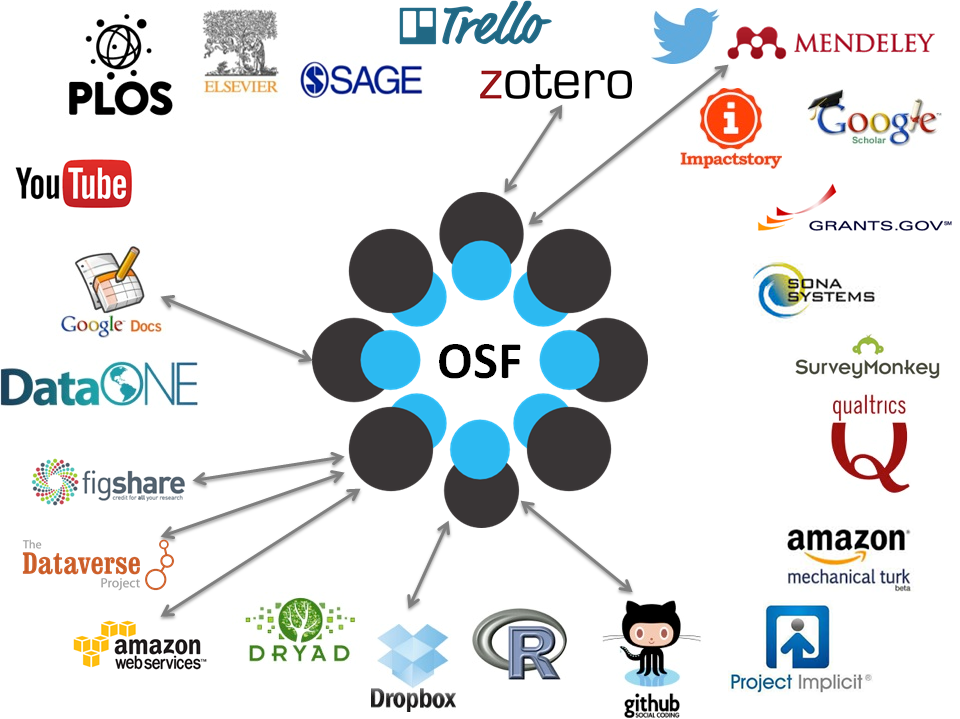
\includegraphics[height=\paperheight]{OSFnow.PNG}
            };
        \end{tikzpicture}
     \end{frame}
 % all template changes are local to this group.
    \setbeamertemplate{navigation symbols}{}
    \begin{frame}[plain]
        \begin{tikzpicture}[remember picture,overlay]
            \node[at=(current page.center)] {
                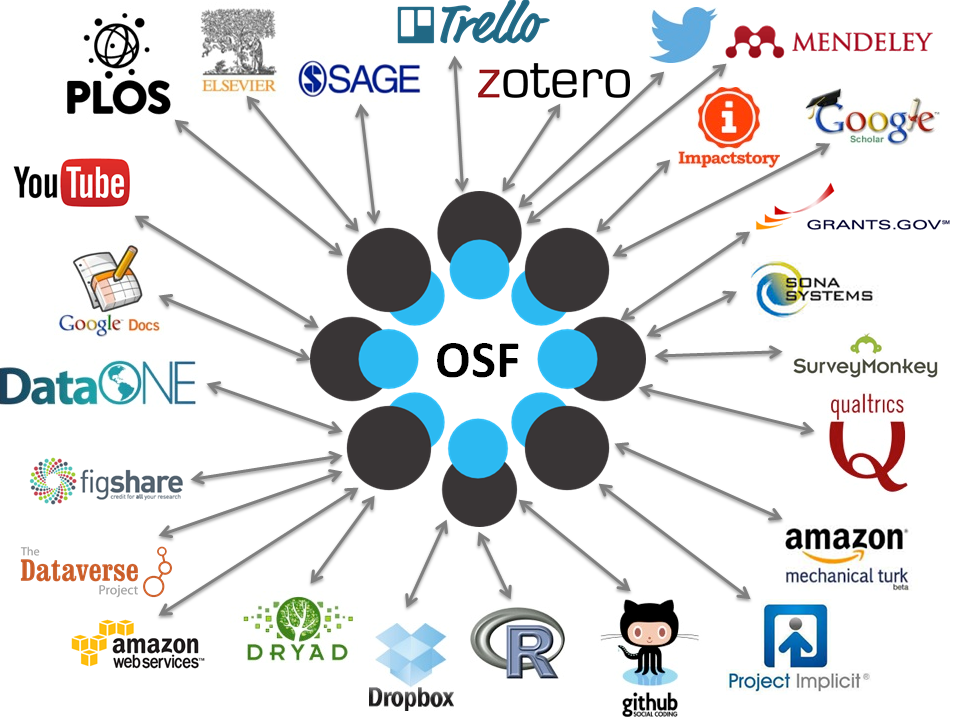
\includegraphics[height=\paperheight]{OSFsoon.PNG}
            };
        \end{tikzpicture}
     \end{frame}
}

\section{Conclusion}
\begin{frame}{Conclusion}
Simple tools exist to help you transparently and reproducibly take your research from beginning to end. 
\begin {itemize}
\item Open Science Framework
\item Trial Registries
\item Version Control
\item Dynamic Documents
\item Trusted Public Data Archive
\end{itemize} 
\vspace{0.25in}
Read more in my \href{http://github.com/garretchristensen/manual}{\textit{Manual of Best Practices in Transparent Social Science Research}} on GitHub.
\end{frame}


\end{document}


